% Template file for an a0 landscape poster.
% Written by Graeme, 2001-03 based on Norman's original microlensing
% poster.
%
% See discussion and documentation at
% <http://www.astro.gla.ac.uk/users/norman/docs/posters/> 
%
% $Id: poster-template-landscape.tex,v 1.2 2002/12/03 11:25:46 norman Exp $


% Default mode is landscape, which is what we want, however dvips and
% a0poster do not quite do the right thing, so we end up with text in
% landscape style (wide and short) down a portrait page (narrow and
% long). Printing this onto the a0 printer chops the right hand edge.
% However, 'psnup' can save the day, reorienting the text so that the
% poster prints lengthways down an a0 portrait bounding box.
%
% 'psnup -w85cm -h119cm -f poster_from_dvips.ps poster_in_landscape.ps'

\documentclass[a0]{a0poster}
% You might find the 'draft' option to a0 poster useful if you have
% lots of graphics, because they can take some time to process and
% display. (\documentclass[a0,draft]{a0poster})
\input defs
\pagestyle{empty}
\setcounter{secnumdepth}{0}
\renewcommand{\familydefault}{\sfdefault}
\newcommand{\QED}{~~\rule[-1pt]{8pt}{8pt}}\def\qed{\QED}

\renewcommand{\reals}{{\mbox{\bf R}}}

% The textpos package is necessary to position textblocks at arbitary 
% places on the page.
\usepackage[absolute]{textpos}

\usepackage{fleqn,psfrag,wrapfig,tikz}

\usepackage[papersize={38in,28in}]{geometry}

% Graphics to include graphics. Times is nice on posters, but you
% might want to switch it off and go for CMR fonts.
\usepackage{graphics}


% we are running pdflatex, so convert .eps files to .pdf
%\usepackage[pdftex]{graphicx}
%\usepackage{epstopdf}

% These colours are tried and tested for titles and headers. Don't
% over use color!
\usepackage{color}
\definecolor{Red}{rgb}{0.9,0.0,0.1}

\definecolor{bluegray}{rgb}{0.15,0.20,0.40}
\definecolor{bluegraylight}{rgb}{0.35,0.40,0.60}
\definecolor{gray}{rgb}{0.3,0.3,0.3}
\definecolor{lightgray}{rgb}{0.7,0.7,0.7}
\definecolor{darkblue}{rgb}{0.2,0.2,1.0}
\definecolor{darkgreen}{rgb}{0.0,0.5,0.3}

\renewcommand{\labelitemi}{\textcolor{bluegray}\textbullet}
\renewcommand{\labelitemii}{\textcolor{bluegray}{--}}

\setlength{\labelsep}{0.5em}


% see documentation for a0poster class for the size options here
\let\Textsize\normalsize
%\def\Head#1{\noindent\hbox to \hsize{\hfil{\LARGE\color{bluegray} #1}}\bigskip}
\def\Head#1{\noindent{\LARGE\color{bluegray} #1}\bigskip}
\def\LHead#1{\noindent{\LARGE\color{bluegray} #1}\bigskip}
\def\Subhead#1{\noindent{\large\color{bluegray} #1}\bigskip}
\def\Title#1{\noindent{\VeryHuge\color{Red} #1}}


% Set up the grid
%
% Note that [40mm,40mm] is the margin round the edge of the page --
% it is _not_ the grid size. That is always defined as 
% PAGE_WIDTH/HGRID and PAGE_HEIGHT/VGRID. In this case we use
% 23 x 12. This gives us three columns of width 7 boxes, with a gap of
% width 1 in between them. 12 vertical boxes is a good number to work
% with.
%
% Note however that texblocks can be positioned fractionally as well,
% so really any convenient grid size can be used.
%
\TPGrid[40mm,40mm]{23}{12}      % 3 cols of width 7, plus 2 gaps width 1

\parindent=0pt
\parskip=0.2\baselineskip

\begin{document}

% Understanding textblocks is the key to being able to do a poster in
% LaTeX. In
%
%    \begin{textblock}{wid}(x,y)
%    ...
%    \end{textblock}
%
% the first argument gives the block width in units of the grid
% cells specified above in \TPGrid; the second gives the (x,y)
% position on the grid, with the y axis pointing down.

% You will have to do a lot of previewing to get everything in the 
% right place.

% This gives good title positioning for a portrait poster.
% Watch out for hyphenation in titles - LaTeX will do it
% but it looks awful.
\begin{textblock}{23}(0,0)
\Title{Money Moves the Pen}
\end{textblock}

\begin{textblock}{23}(0,0.6)
{
\LARGE Link Prediction in Congress Bill Co-Sponsorship Networks Using Political Donor Network Information
}

{
\Large
\color{bluegray}
\emph{Yi Zhong, Eddie Chen || CS224W Fall 2018 II Class Project}
}
\end{textblock}

% Uni logo in the top right corner. A&A in the bottom left. Gives a
% good visual balance, but you may want to change this depending upon
% the graphics that are in your poster.
\begin{textblock}{2}(17,0)
%Your logo here

\includegraphics[width=6in]{CS-Logo-horizontal}
\end{textblock}

%\begin{textblock}{2}(21.2,0)
%Another logo here
%%\resizebox{2\TPHorizModule}{!}{\includegraphics{/usr/local/share/images/GUVIu/GUVIu.eps}}
%\end{textblock}


\begin{textblock}{7.0}(0,1.5)

\hrule\medskip
\Head{Introduction}\\
Political collaboration is an important part of legislative life, and congress bill cosponsorships provide a rich source of information about the social network between legislators, and serving as a proxy to understand legislators' "connectedness" and collaboration graph. Moreover, according to Mark Twain, "we have the best government that money can buy" - money and politics have already been intertwined. In this project, we applied social network analysis tools on political donation networks and congress bill cosponsorship networks, and framed our research problem as a link prediction task on congress bill cosponsorship networks using political campaign donation records for the US (Congress and Presidential Campaigns) with its network characteristics. We modeled and presented graph characteristics of the two political networks, and showed investigation results of link prediction using various supervised learning techniques for this project. We then compared models' performance to a naive baseline to come up with evaluations. 

\medskip
\hrule\medskip
\Head{Method}\\
Our project is made up of two parts: graph modeling, and link prediction. For graph modeling, we aim to construct a tripartite graph of political committees, legislators (we will ignore those failed to get elected to office), and the bills those legislators worked together on. A sample graph can be found in Figure \ref{fig_sim}. With the graph constructed, we provide a set of statistics and descriptions of the graph structure (including their one-mode projections, for both bills-legislators and committees-legislators subgraphs). After that, we construct a link prediction problem by dividing graph into different years of congress, and select the suitable years for model training and evaluation. Lastly, we report our learnings from the entire exercise. 

\begin{figure*}[!t]
\centering
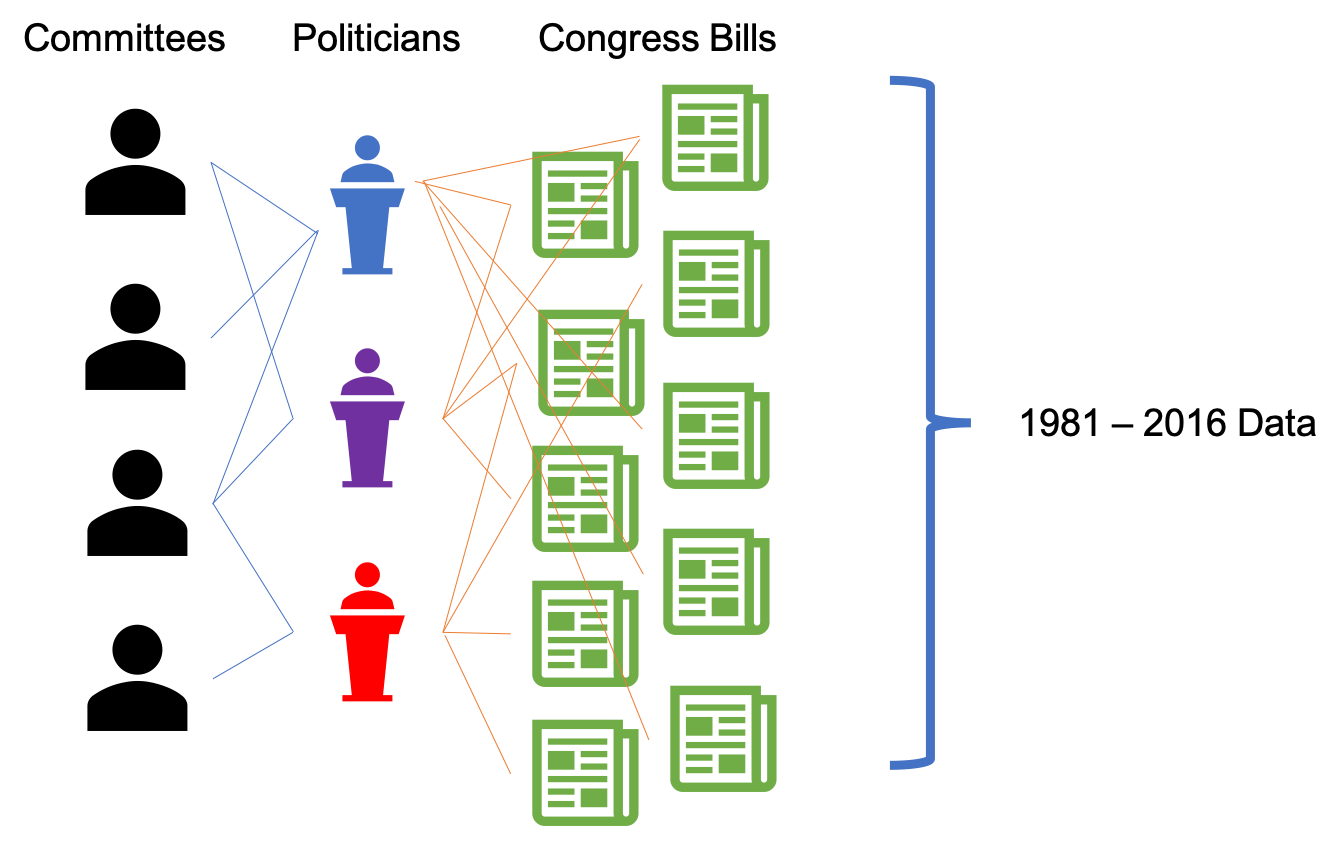
\includegraphics[width=5in]{network_illustration2}
\caption{Illustration of the Congress Political Network}
\label{fig_sim}
\end{figure*}


\medskip
\hrule\medskip
\Head{Link Prediction}\\
We frame our link prediction problem as follows: predict the link between legislators, where a link exists if two legislators cosponored a bill together, for a specific Congress term.  

We have constructed three link prediction models:
\begin{itemize}
    \item Naive baseline predictor: a baseline model based on graph density
    \item Legislator only predictor: a baseline model based on candidate attributes (party, state)
    \item Campaign only predictor: prediction model using features generated from campaign graph network attributes
\end{itemize}

\end{textblock}

\begin{textblock}{7.0}(8,1.5)
\hrule\medskip
\Head{Features and Algorithms}\\
We constructed features from the campaign subgraph for Campaign only predictor. Features include: 
\begin{itemize}
\item Common Neighbors, Union of Neighbors, Jaccard Index
\item Degree Difference in a pair of legislator nodes
\item Contribution Amount (sum and absolute difference)
\item Clustering Co-efficient (sum, absolute difference, mean)
\item Degree Centrality difference
\item Shortest Distance between two legislator nodes
\item Spectral Clusters from Clauset-Newman-Moore greedy modularity maximization
\item node2vec embeddings
\end{itemize}
For features used in the Legislator only predictor, we collected legislators' affiliated party and home state information, by term. 

For algorithms, we used supervised learning models like \textbf{logistic regression} and \textbf{decision trees}. For logistic regression, we used scikit-learn's default implementation with {-1,1} notation for labels and $L2$ regularization. A decision tree is a tree where each node represents a feature, each branch represents a decision/rule and each leaf represents a classification in our case. We used Scikit Learn's default implementation which uses Gini Index as the metric

\medskip
\hrule\medskip
\Head{Evaluation Method}\\
We used accuracy as our main success measure: $$Accuracy = \frac{NumberOfCorrectPredictions}{TotalNumberOfPredictionsMade}$$

We define our \textbf{naive baseline predictor} as follows: given a pair of nodes$v_1, v_2$, we will always predict there will be an edge between these two pairs, i.e. as a complete graph. That is, $$Accuracy_{Naive Baseline} = \frac{2||E||}{||V|| \dot (||V|| - 1)} $$

Using the 100th Congress (1987 - 1988) as the training set and the 101th Congress (1989-1990) as the test set. The baseline accuracy is calculated as $96,052/138,075= 0.695$.

\medskip
\hrule\medskip
\Head{Results and Findings}\\
The basic stats of the tripartitie graph are included below: 
\begin{itemize}
\item Legislator count: 1,919 (1813 of which are found in campaign financial network)
\item Bill count: 221,726 
\item Committee count: 14,326
\item Edges between legislators and bills: 3,086,039
\item Edges between committees and candidates: 911,965
\item Overall tripartite graph node count: 237,971, and edge count: 3,998,004
\end{itemize}

\end{textblock}

\begin{textblock}{7.0}(16,0.8)

\hrule\medskip
\Head{Network Description}
\begin{figure}
\centering
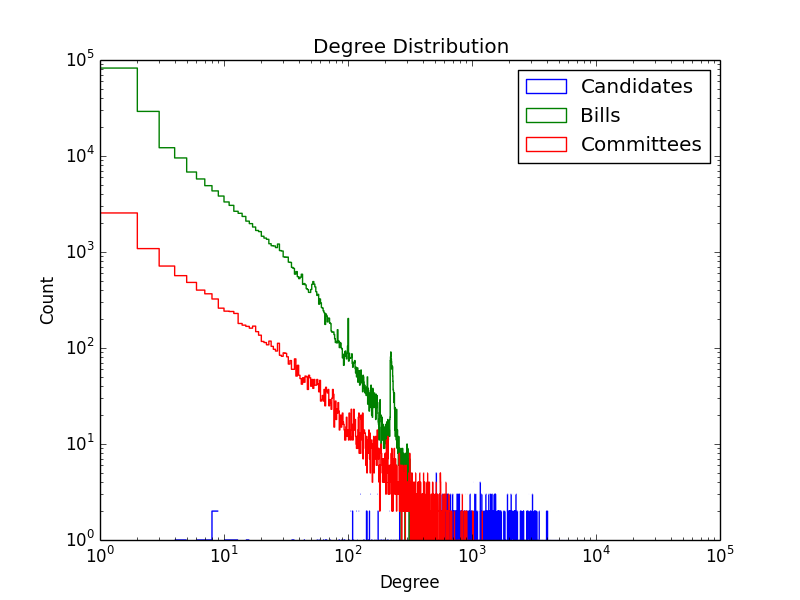
\includegraphics[width=0.4\linewidth]{overall_deg_distro}
\caption{Overall Tripartite Graph Degree Distribution on log-log scale}
\label{fig:overalldegdistro}
\end{figure}
\textbf{Bill Co-authorship Graph resembles the academic collaboration graph with a power law pattern} (long tail) - the most frequent degrees are the smallest degrees, and it has a very high clustering co-efficient. 
For the \textbf{folded campaign contribution graph, it represents a typical small world pattern with high clustering coefficient}.

\medskip
\hrule\medskip
\Head{Model Performance}
\begin{table}[htb]
%\resizebox{\columnwidth}{!}{

\begin{tabular}{|l|r|r|}

\hline
\multicolumn{1}{|c|}{Model} & \multicolumn{1}{c|}{Train Accuracy} & \multicolumn{1}{c|}{Test Accuracy} \\ \hline
1 - Naive Baseline  & 0.695      & 0.695         \\ \hline
2 - Candidate Party/State, Logistic Regression  & 0.695      & 0.698         \\ \hline
3.1 - Campaign only, Logistic Regression & 0.786      & 0.774         \\ \hline
3.2 - Campaign only, Decision Tree & 0.854      & 0.794         \\ \hline
3.3 - Campaign only, Logistic Reg w/ node2Vec & 0.728      & 0.728         \\ \hline
\end{tabular}
%}
\caption{Model Performance for Limited Dataset}
  \label{tab:model1}
\end{table}

\begin{table}[htb]
%\resizebox{\columnwidth}{!}{
\begin{tabular}{|l|r|r|}

\hline
\multicolumn{1}{|c|}{Model} & \multicolumn{1}{c|}{Train Accuracy} & \multicolumn{1}{c|}{Test Accuracy} \\ \hline
1 - Naive Baseline  & 0.697      & 0.691         \\ \hline
2 - Candidate Party/State, Logistic Regression  & 0.695      & 0.698         \\ \hline
3.1 - Campaign only, Logistic Regression & 0.748      & 0.714         \\ \hline
3.2 - Campaign only, Decision Tree & 0.795      & 0.740         \\ \hline
\end{tabular}
%}
\caption{Model Performance for All Datasets Combined}
  \label{tab:model2}
\end{table}

\begin{figure}
\centering
\begin{minipage}{0.48\linewidth}

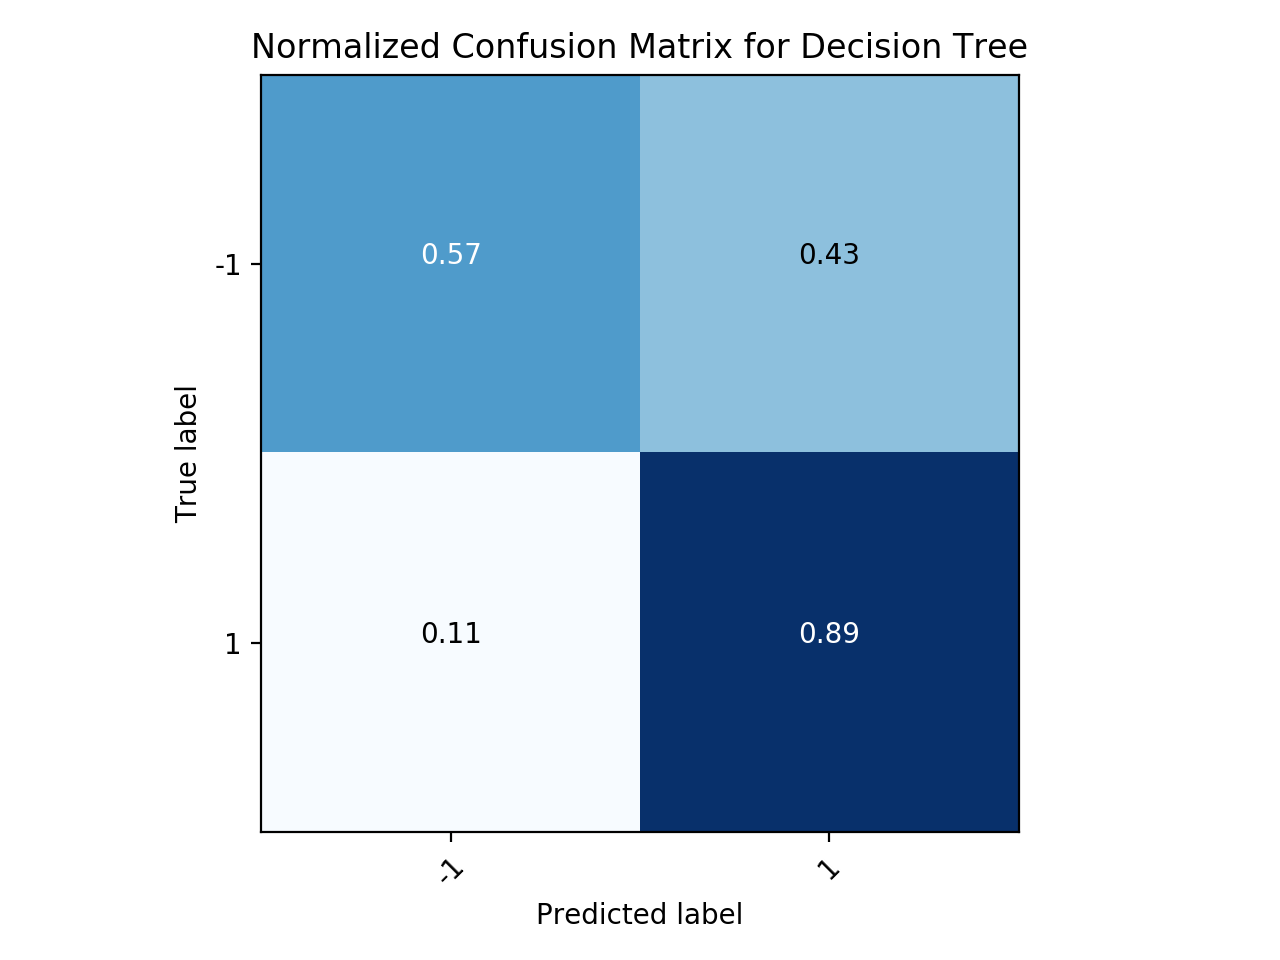
\includegraphics[width=\linewidth]{confusion_tree_limited}
\caption{Confusion Matrix for Decision Tree in Limited Dataset}
\label{fig:confusion_tree_limited}
\end{minipage}\hfill
\begin{minipage}{0.48\linewidth}

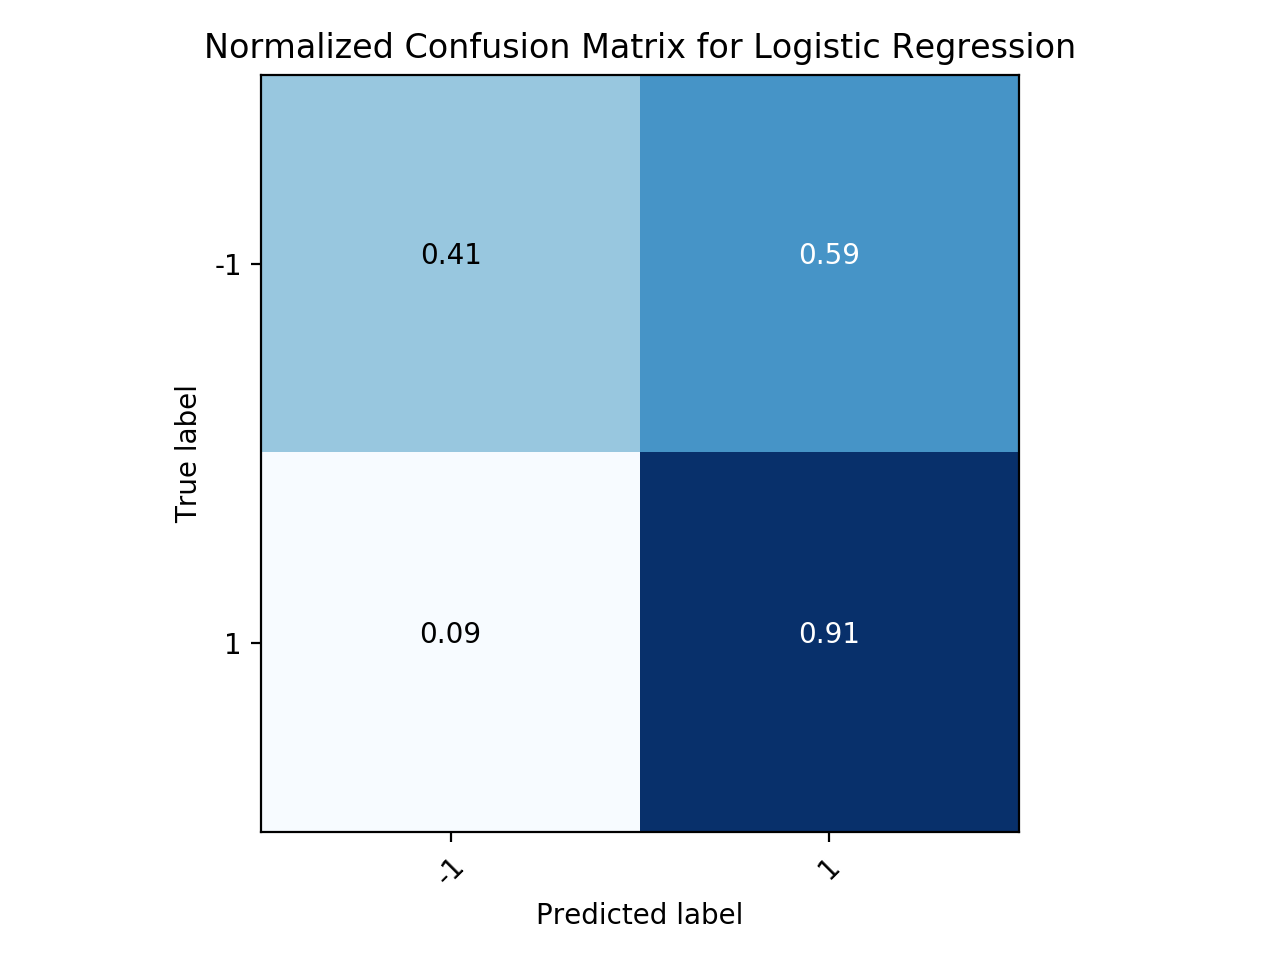
\includegraphics[width=\linewidth]{logreg_limited}
\caption{Confusion Matrix for Logistic Regression in Limited Dataset}
\label{fig:logreg_limited}
 \end{minipage}
\end{figure}

\medskip
\hrule \medskip
\Head{Conclusion}\\
US Congressional Politics is indeed a small world: legislators are connected to other legislators via common donors and co-authorship on bills. We have identified the academic collaboration network-like pattern for bill co-authorship data, and a "small world" pattern among legislators, with consistently high clustering coefficients. Moreover, it does appear that "money moves politics": using features learned from campaign donation networks, we can confidently predict if two legislators will later collaborate on bills together - beating a naive baseline. In paricular, decision tree model performed very well to give us $79\%$ accuracy. 

\end{textblock}

\end{document}
